% !TeX root = prob.tex

\section{Gambler's Ruin}\label{s.gamblers}

\textbf{Problem} Two players $A$ and $B$ compete in a contest. There is an initial finite capital of $n$ units: $A$ has $i$ and $B$ has $n-i$. They repeated play a game such that the probability that $A$ wins is $p$ and the probability that $B$ wins is $q=1-p$. The loser gives one unit to the winner. When one player has $n$ units the contest is finished.
\begin{enumerate}
\item Given initial parameters $(p, n, i)$, what is the probability that $A$ wins?
\item What is the expectation of the duration of the game?
\end{enumerate}
%\begin{figure}[tb]
\begin{center}
\begin{tikzpicture}[scale=1.2]
\draw (0,0) node[above left] {$A$} -- 
      (10,0) node[above right] {$B$};
\foreach \x in {0,1,2,3,4,5,6,7,8,9,10} {
  \draw (\x,0) -- +(0,4pt);
  \node at (\x,-10pt) { $\x$ };
}
\node at (4,-9mm) {$i$};
\node at (10,-9mm) {$n$};
\draw[fill] (4,7mm) circle[radius=1pt];
\draw[->] (4,7mm) -- node[above] {$q$} +(-1,0);
\draw[->] (4,7mm) -- node[above] {$p$} +(1,0);
\end{tikzpicture}
\end{center}
%\caption{What is the probability that the particle reaches $0$ or $n$?}\label{f.ruin3}
%\end{figure}
The gambler's ruin is presented in most books on probability such as \cite[Section~2.7.2]{BW}, \cite[Section~3.4]{ross},\cite{mosteller}, \cite{mos}. \cite[Chapter~2]{privault} has a more extensive discussion which includes the solution to the expectation of the duration of the contest.\footnote{Privault presentation asks for the probability that $A$ is ruined, that is, that $B$ wins. I follow other references who ask for $A$'s probability of winning.}

\subsection{Theoretical solutions}

Given $(p,n,i)$ the probability that $A$ wins the contest is:
\[
P_A(p, n, i) = \left(\frac{1-r^{i}}{1-r^n}\right)\,,
\]
where $r=q/p$. By symmetry, the probability that $B$ wins is:
\[
P_B(p, n, i) = \left(\frac{1-(1/r)^{n-i}}{1-(1/r)^{n}}\right)\,.
\]

There are separate solutions for $p\neq 1/2$ and $p=1/2$. For $p\neq 1/2$ the expectation of the duration of the contest is:
\[
P_{\mathit{duration}}(p,n,i)=\frac{1}{q-p}\left(i-n
\frac{1-r^k}{1-r^n}\right)\,.
\]
For $p=1/2$ the expectation of the duration of the contest is:
\[
P_{\mathit{duration}}(p,n,i)=i(n-1)\,.
\]
Of course the duration does not depend on which player wins. If $A$ wins, the contest terminates for $B$ also, and conversely.

\subsection{Program structure}

The program is divided into three modules:
\begin{itemize}
\item \verb+configuration.py+ contains declarations of variables which are intended to be constants.
\item \verb+gambler_plot.py+ contains the functions for plotting the histogram of the duration of the contests. If the simulation is run for multiple probabilities or initial values, a graph of the probability of wins is also displayed. The module imports \verb+matplotlib.pyplot+.
\item \verb+gamblers_ruin.py+ is the main program which obtains the parameters, runs the simulations and prints the output.
\end{itemize}

\subsection{Running the simulations}

The program runs the simulations in a loop, each time asking the user how to run it. You can run the same simulation again with the saved parameters, enter new parameters, or run a sequence of simulations for a range of probabilities or initial values.

A typical output is as follows:
\begin{verbatim}
Probability = 0.450, capital = 20, initial = 10
Wins = 127, losses = 873, limits exceeded = 0
Proportion of wins     = 0.1270
Probability of winning = 0.1185
Average duration  = 78
Expected duration = 76
\end{verbatim}
The results of the simulation are very close to the theoretical probability and duration.

Figure~\ref{f.gambler-hist1} shows the histogram for the duration of the contest, limited to a duration of $200$. The vertical line is the expectation.
\begin{figure}
\begin{center}
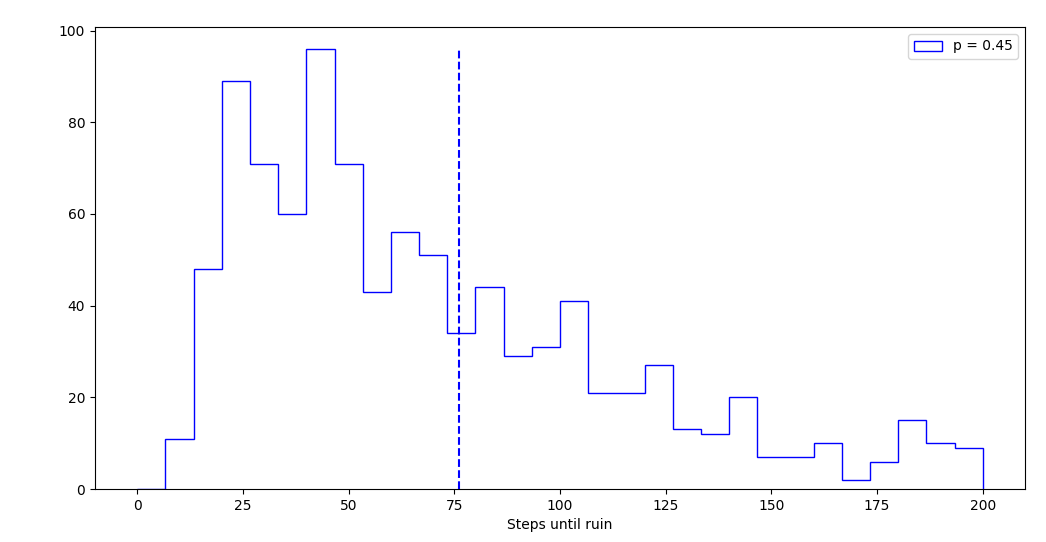
\includegraphics[width=\textwidth]{gamblers_ruin-01}
\end{center}
\caption{Histogram for $p=0.45, n=20, i=10$}\label{f.gambler-hist1}
\end{figure}

Figure~\ref{f.gambler-hist2} proportion of wins for multiple probabilities. It also shows histograms for the duration of the contest for these probabilities. 
\begin{figure}
\begin{center}
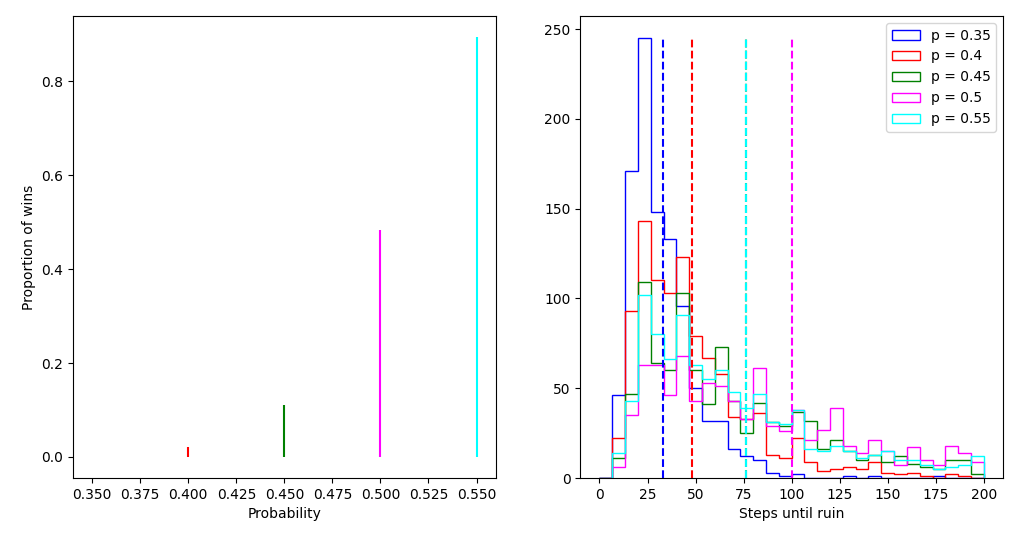
\includegraphics[width=\textwidth]{gamblers_ruin-02}
\end{center}
\caption{Proportion of wins and histogram for $n=20, i=10$ and multiple probabilities}\label{f.gambler-hist2}
\end{figure}

\subsection{Technical notes}

When the simulation is run for the first time in Visual Studio Code, you must click on the terminal window (or \verb+ctrl `+) to enter the parameters.

When the simulation is run multiple times, the program closes each figure and replaces it with the new one. This does not work on some Python environments such as IDLE and Thonny. Change the configuration constant \verb+CLOSE+ to true. You will now have to close each figure before running a new simulation.
